\documentclass{article}
\usepackage{graphicx}
\usepackage [dvipsnames] {xcolor}
\graphicspath{ {./images/} }

\begin{document}

%TITLE PAGE

  \begin{titlepage}

%LOGO
    \begin{center}
    
\includegraphics[height=5cm]{Logo_Polimi}\\
    \vspace{7cm}
      \begin{huge}
        \textbf{CLup - Customer Line Up}\\
      \end{huge}
      \vspace{0.3cm}
      \begin{large}
        \textit{Software Engineering 2 Project 2020/21}\\
      \end{large}
      
      \vfill
      \begin{author}
        \textbf{\Large Authors}\\
        \begin{itemize}
          \item Francesco Attorre - \textit{10618456}\\
          \item Thomas Jean Bernard Bonenfant - \textit{10597564}\\
          \item Veronica Cardigliano - \textit{10627267}\\
        \end{itemize}
      \end{author}

    \end{center}
  
  \end{titlepage}
  
  
    \section{Introduction}
    	\renewcommand{\thesubsection}{\Alph{subsection}}
     	\subsection{Purpose}
	The goal of this document (RASD: Requirements Analysis and Specification Document) is to describe a model of the proposed     	problem capturing the main aspects of it, analyzing its requirements, goals, actors, domain assumptions, scenarios and relative 	use cases. This document is addressed to the developers of the software to be, to give a simplified view of it. 
	This specific problem has the goal of  developing an easy application to allow store managers to regulate the influx of people in the 	building and to prevent the customers from having to line up outside stores for a long time.

         \subsection{Scope}
         \subsubsection {Description of the given problem}
         In a period of global pandemic, a lot of usually normal actions have become challenges, first of all the common entry into a public 	place like a supermarket. In this context, CLup digitalizes ticket numbers distribution giving customers the opportunity to queue and 	to plan store visits from home. This allows people to save time and be safer, and store managers to better control and limit the 		accesses to the building. This will be obtained scanning the QR codes generated by the app for each incoming customer, that will 	allow also to take track of who entered the store, when he entered and of other people present at that time.
	About shared phenomena, customers will have the opportunity to register to the app in order to have customized services, such as 	average time spent in the shop, and the possibility to book a visit in a specific time slot. When it’s time for them to leave for the 		building, they’ll be noticed based on how far they are, to avoid that they leave too early or late creating again the unwanted queues 	in front of the building.
	Planning store visits, customers will have the possibility to indicate the expected permanence time and the departments from which 	they intend to buy, in order to understand where they’re gonna spend their time and to be able to better distribute them.

         \subsubsection {Current system}
         So far, people who want to access a building have to take a ticket on site, this means a lot of time spent waiting in queue and risking being infected. CLup was designed to avoid this taking advantage of technological tools.
However, as well as booking from home, customers unable to use the app can also take a ticket on the spot, which will be registered in the app by the store manager. In this way the previous technology integrates with the new one avoiding to exclude anyone from the possibility of entering the building.
         
         \subsubsection{Goals}
         \renewcommand{\theenumi}{[G\,\arabic{enumi}]}
	 \begin{enumerate} 
         	\item Allow an Activity to register to CLup.
		\item Allow an Activity to insert one or more Buildings.
		\item Allow Store Managers to sign up for a Building.
		\item Allow an AppCustomer to register to CLup.
		\renewcommand{\labelenumii}{\theenumii}
		\renewcommand{\theenumi}{G\,\arabic{enumi}}
		\renewcommand{\theenumii}{[\theenumi.\arabic{enumii}].}
		\begin{enumerate}
			\item Allow a RegisteredAppCustomer to login.
		\end{enumerate}
		\renewcommand{\theenumi}{[G\,\arabic{enumi}]}
		\item Allow an AppCustomer to choose a Building to visit.
		\renewcommand{\labelenumii}{\theenumii}
		\renewcommand{\theenumi}{G\,\arabic{enumi}}
		\renewcommand{\theenumii}{[\theenumi.\arabic{enumii}].}
		\begin{enumerate}
			\item Allow a RegisteredAppCustomer to login.
			\item Allow a RegisteredAppCustomer to choose a Building to book for.
			\item Allow AppCustomers to view Buildings at a certain distance from their position. 
			\item Allow AppCustomers to view estimated TravelTime to reach a Building.
		\end{enumerate}
		\renewcommand{\theenumi}{[G\,\arabic{enumi}]}
		\item Allow AppCustomers to know when they should leave for the Building.
		\item Allow a Customer to acquire a Ticket.
		\renewcommand{\labelenumii}{\theenumii}
		\renewcommand{\theenumi}{G\,\arabic{enumi}}
		\renewcommand{\theenumii}{[\theenumi.\arabic{enumii}].}
		\begin{enumerate}
			\item Allow an AppCustomer to line up to access a Building. 
			\item Allow a RegisteredAppCustomer to book a visit to a Building.
			\item Allow a PhysicalCustomer to acquire a PhysicalTicket.
		\end{enumerate}
		\renewcommand{\theenumi}{[G\,\arabic{enumi}]}
		\item  Allow Customers to enter the Building when it’s their turn.
		\renewcommand{\labelenumii}{\theenumii}
		\renewcommand{\theenumi}{G\,\arabic{enumi}}
		\renewcommand{\theenumii}{[\theenumi.\arabic{enumii}].}
		\begin{enumerate}
			\item Allow StoreManagers to monitor entrances scanning a QR code for each AppCustomer willing to enter the Building.
			\item Allow StoreManagers to monitor entrances of PhysicalCustomers when it’s their turn to enter the Building.
		\end{enumerate}
		\renewcommand{\theenumi}{[G\,\arabic{enumi}]}
		\item Allow a StoreManager to enter LineUpDigitalTickets.
		\item Allow each AppCustomer to see a list of acquired DigitalTickets.
		\item Allow StoreManagers to inform CLup when a Customer leaves a Building.
		\renewcommand{\labelenumii}{\theenumii}
		\renewcommand{\theenumi}{G\,\arabic{enumi}}
		\renewcommand{\theenumii}{[\theenumi.\arabic{enumii}].}
		\begin{enumerate}
			\item Allow StoreManagers to read an exit QR code.
		\end{enumerate}
	\end{enumerate}
         
         \subsection{Definitions, Acronyms, Abbreviations}
         	\subsubsection{Definitions}
		\begin{itemize}
			\item \textcolor{BrickRed}{Digital Ticket}: Digital counterpart of a usual Ticket Number. It contains the date (including time) of its reservation, the identifier of the Building the Customer wishes to visit and the number to add in the priority queue.
			\item \textcolor{BrickRed}{LineUpDigitalTicket}: a Digital Ticket that also contains the number added in the priority queue. If it is requested by a StoreManager it will be associated to the number of the Physical Ticket given to a PhysicalCustomer
			\item \textcolor{BrickRed}{BookingDigitalTicket}: a Digital Ticket that contains also the date and time of arrival and estimated leaving and optionally the Departments of the Building that the RegisteredAppCustomer chose.
			\item \textcolor{BrickRed}{Building}: physical place managed by an activity registered to the system where customers can enter.
			\item \textcolor{BrickRed}{Physical Ticket}: Ticket from a Ticket Dispenser. When collected the number written on it is associated with a new Digital Ticket by the System. (This process is initiated by the Store Manager who notifies the system that he collected a Physical Ticket
			\item \textcolor{BrickRed}{EstimatedPermanenceTime}: for a Booking is the difference between selected Exit Time and selected Arrival Time.
			\item \textcolor{BrickRed}{Waiting Time}: The estimated time the Customer must wait in order to enter the Building.
			\item \textcolor{BrickRed}{Arrival Time}: when the Customer reaches the Building
			\item \textcolor{BrickRed}{Exit Time}: when the Customer exits the Building
			\item \textcolor{BrickRed}{ValidDigitalTicket}: DigitalTicket state that grants its owner access to the Building.
			\item \textcolor{BrickRed}{NotValidDigitalTicket}: DigitalTicket’s owner cannot enter the Building yet.
			\item \textcolor{BrickRed}{ExpiredDigitalTicket}: DigitalTicket that doesn’t grant access to the Building (neither in the future with the same DigitalTicket). Expected time to enter (fixed on the DigitalTicket) + 15 minutes > actual time.
			\item \textcolor{BrickRed}{BuildingAccessCode}: Building’s secret code which allows Store Managers to sign up for the associated Building.
			\item \textcolor{BrickRed}{TravelTime}: Time needed to reach the Building according to the selected means of transport. Therefore a means of transport must be selected in order to compute it.
			\item \textcolor{BrickRed}{Department}: a Building is composed of one or more zones called Departments.
			\item \textcolor{BrickRed}{BuildingCapacity}: number of Customers generally allowed in the store. In case of more than one Department, this number takes into account the smallest department, to ensure that crowds are avoided.
			\item \textcolor{BrickRed}{BookingCapacity}:  40\% of BuildingCapacity 
			\item \textcolor{BrickRed}{DepartmentSurplus}: extra Customers allowed in a specific Department, when it is larger than the base one.
			\item \textcolor{BrickRed}{TimeSlot}: time interval multiple of 15 minutes with a starting time. They include all the opening time of the store and each RegisteredAppCustomer can book one of them
			\item \textcolor{BrickRed}{AvailableTimeSlot}: according to the Customer choices(date, EstimatedPermanenceTime, Departments), a TimeSlot is available if the number of RegisteredAppCustomers who have booked is less than the BookingCapacity or one of the DepartmentSurplus of the chosen Departments has not been reached yet. In AvailableTimeSlot, RegisteredAppCustomer can book a visit.
		\end{itemize}
		
		\subsubsection{Acronyms}
		\begin{itemize}
			\item \textcolor{BrickRed}{RASD}: Requirements Analysis and Specification Document 
			\item \textcolor{BrickRed}{QR code}: Quick Response code, a 2D barcode typically used to store information intended to be read using a smartphone.
			\item \textcolor{BrickRed}{GPS}: Global Positioning System
			\item \textcolor{BrickRed}{CLup}: Customers Line-up
			\item \textcolor{BrickRed}{DD}: Design Document 
		\end{itemize}
		
		\subsubsection{Abbreviations}
		\begin{itemize}
			\item \textcolor{BrickRed}{Gn}: goal number n
			\item \textcolor{BrickRed}{Rn}: requirement number n
			\item \textcolor{BrickRed}{Dn}: domain number n
		\end{itemize}
		
	\subsection{Revision History}
	\subsection{Reference Documents}
	\begin{itemize}
			\item \textcolor{BrickRed}{Specification Document}: “R\&DD Assignment AY 2020-2021.pdf”
			\item \textcolor{BrickRed}{Slides of the lectures}
			\item \textcolor{BrickRed}{Alloy Doc}: domain number n
	\end{itemize}
	
	\subsection{Document Structure}
	...
	
	\section{Overall Description}
	\subsection{Product Perspective}
	\subsubsection{Scenarios}
	{\large{Scenario 1 - Line up for a building}} \\
	\\
	John needs to go to the nearest grocery store. So he opens the CLup application, chooses to go on foot, but he notices that the nearest grocery store has an estimated waiting time of 30 min plus it takes him 5 min to get there. Then he notices that a store a little further has an estimated waiting time of 12 min plus it takes him 10 min to get there, so he requests a digital ticket to line up and leaves home.
When he gets to the store he waits in line until it’s his turn, opens the application and presents the QR Code associated with his digital ticket to the Store Manager.
The Store manager scans the QR Code from his application and receives a “Ticket accepted” notification, so he lets the Customer in.
After an hour of shopping, John leaves the grocery store. \\
\\
	{\large{Scenario 2 - book a visit to a building}} \\
	\\
	Tomorrow Bob plans to go to the grocery store, but he can only go at 4 pm as he needs to be back to work at 5 pm. Because of this, he opens the CLup app, registers for the first time and logs in with his credentials (username and password).Bob sets the car as mean of transport and chooses the first Store of the list that the app shows him, which is also the nearest, booking a visit from 4 pm to 5 pm, with an estimated time of one hour and without choosing specific categories of items.
The following day he reaches the store in time presenting the QR Code associated with his booking. The store manager scans his QR Code, receives a “Ticket Accepted” notification and lets Bob in.
Bob’ll show again a QR code to certify the end of the shopping at exactly 4:49 pm before leaving the building. \\
\\
	{\large{Scenario 3 - Physically line up to enter a building} }\\
	\\
	It’s 8:30 am. The Store will open at 9 am. The Store Manager has to prepare the Ticket Dispenser for Customers who don’t use the CLup application. He refills the Ticket Dispenser paying attention to the initial ticket number and the last ticket number. He then opens his CLup application, logs in, selects “Initialize Ticket Dispenser'' and inserts the Initial Ticket Number and the last Ticket Number. \\
	\\
	{\large{Scenario 4 - A blackout has occurred} }\\
	\\
	Veronica, looking at her empty fridge, decides to go to a supermarket to buy some food. She decides to use the CLup, and, being very hungry, she wants to reach the nearest Supermarket, 10 minutes far from her home by car, as soon as possible.
Veronica opens the App, sets her features and chooses the first choice, asking for a Digital Ticket to LineUp.
The CLup service gives Veronica the number 5, and shows her that the next number is 3. Based on the average time spent in the supermarket, CLup will notice her when to leave for the supermarket.
After being notified, Veronica leaves from home and arrives in front of the building.
She waits 5 minutes for a customer to pay and leave, then she shows the QR code on the CLUp app to the Store Manager in the entrance and enters the building to do half an hour of shopping. 
Unluckily, during the shopping a blackout occurs, so people in the queue receive an error message in CLup, notifying them that the store had to close due to an unexpected problem. Veronica has to leave her shopping and order takeaway. \\
\\
	{\large{Scenario 5 - small mistake, wrong building}} \\
	\\
	Jane wants to do shopping before her smart working begins, at 9 o’ clock, then opens CLup as soon as she wakes up. She sets a maximum distance of 2 km and “by car” as means of transport, and chooses the first shop in the list. She’s the only one in line, so CLup notifies her immediately to leave for the building. Jane, then, leaves home quickly, but she is still a little asleep, so she reaches the wrong Building. Also such Building has just opened, so also there it's up to number 1. The Store Manager scans her QRcode and receives a “Ticket denied'' Notification, so he prevents Jane from entering. At this point she realizes the mistake and goes to the right shop, but it is quite far, so when she arrives her ticket has already expired. \\
	\subsubsection{Class Diagrams}
	\large{Actors - Class Diagram} \\
	\\
	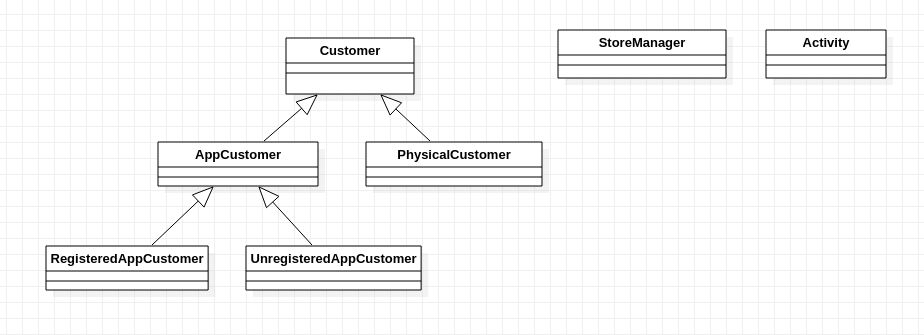
\includegraphics[height=4cm]{ActorsClassDiagram}\\
	\\
	\\
	\large{Overall Class Diagram} \\
	\\
	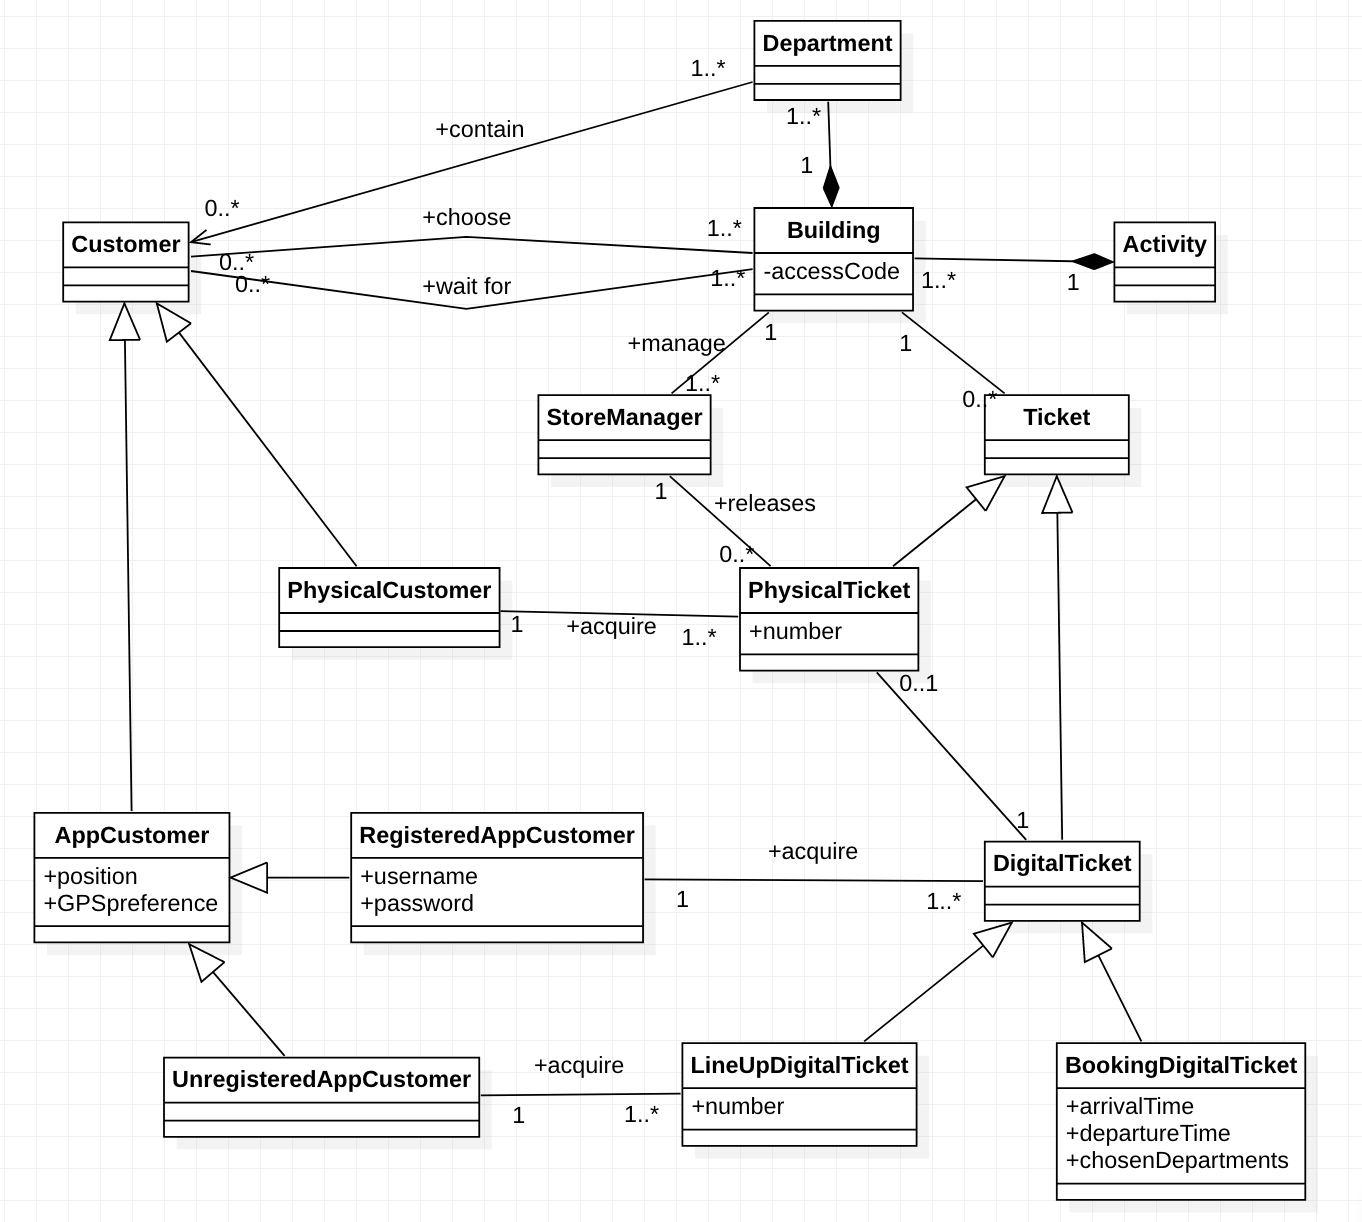
\includegraphics[height=10cm]{ClassDiagram}\\
	\\
	\large{State Charts} \\
	\\
	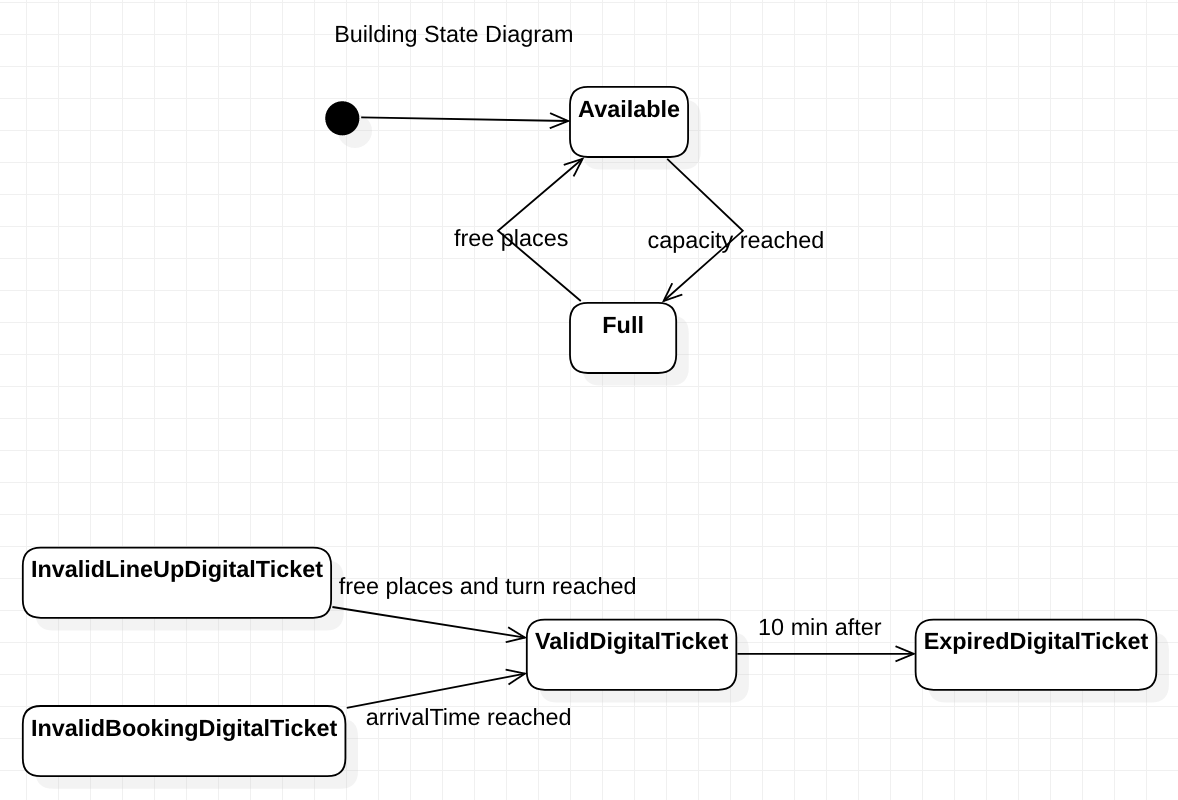
\includegraphics[height=6cm]{StateDiagram}\\
	
	\subsection{Product Functions}
	In this section we include the most important Requirements with which each Goal, that represents different world phenomena that CLup aims to manage, can be satisfied. The requirements represent shared phenomena, which could be controlled by the world and observed by the machine or vice versa, but in each case they involve both the system, CLup, and the external world, in our case Customers, Activities and Store Managers. We have given prominence to this section in order to clarify any ambiguity of the assignment and make future developments of CLup as simple as possible.
		
	\subsubsection{Requirements}
	
	 \renewcommand{\theenumi}{[G\,\arabic{enumi}]}
	 \begin{enumerate}
	 \color{BrickRed}
	 	\item Allow an Activity to register to CLup.
		\renewcommand{\labelenumii}{\theenumii}
		\renewcommand{\theenumi}{G\,\arabic{enumi}}
		\renewcommand{\theenumii}{[\theenumi.\arabic{enumii}].}
		\begin{enumerate}
			\item Allow an Activity to log in
		\end{enumerate}
		\renewcommand{\theenumi}{[G\,\arabic{enumi}]}
		\item Allow an Activity to insert one or more Buildings.
		\item Allow Store Managers to sign up for a Building.
		\item Allow an AppCustomer to register to CLup.
		\renewcommand{\labelenumii}{\theenumii}
		\renewcommand{\theenumi}{G\,\arabic{enumi}}
		\renewcommand{\theenumii}{[\theenumi.\arabic{enumii}].}
		\begin{enumerate}
			\item Allow a RegisteredAppCustomer to login.
		\end{enumerate}
		\renewcommand{\theenumi}{[G\,\arabic{enumi}]}
		\item Allow an AppCustomer to choose a Building to visit.
		\renewcommand{\labelenumii}{\theenumii}
		\renewcommand{\theenumi}{G\,\arabic{enumi}}
		\renewcommand{\theenumii}{[\theenumi.\arabic{enumii}].}
		\begin{enumerate}
			\item Allow an AppCustomer to choose a Building to line up for.
			\item Allow a RegisteredAppCustomer to choose a Building to book for.
			\item Allow AppCustomers to view Buildings at a certain distance from their position.
			\item Allow AppCustomers to view estimated TravelTime to reach a Building.
		\end{enumerate}
		\renewcommand{\theenumi}{[G\,\arabic{enumi}]}
		\item Allow AppCustomers to know when they should leave for the Building.
		\item Allow a Customer to acquire a Ticket.
		\renewcommand{\labelenumii}{\theenumii}
		\renewcommand{\theenumi}{G\,\arabic{enumi}}
		\renewcommand{\theenumii}{[\theenumi.\arabic{enumii}].}
		\begin{enumerate}
			\item Allow an AppCustomer to line up to access a Building.
			\item Allow a RegisteredAppCustomer to book a visit to a Building.
			\item Allow a PhysicalCustomer to acquire a PhysicalTicket.
		\end{enumerate}
		\renewcommand{\theenumi}{[G\,\arabic{enumi}]}
		\item Allow Customers to enter the Building when it’s their turn.
		\renewcommand{\labelenumii}{\theenumii}
		\renewcommand{\theenumi}{G\,\arabic{enumi}}
		\renewcommand{\theenumii}{[\theenumi.\arabic{enumii}].}
		\begin{enumerate}
			\item Allow StoreManagers to monitor entrances scanning a QR code for each AppCustomer willing to enter the Building.
			\item Allow StoreManagers to monitor entrances of PhysicalCustomers when it’s their turn to enter the Building.
		\end{enumerate}
		\renewcommand{\theenumi}{[G\,\arabic{enumi}]}
		\item Allow a StoreManager to enter LineUpDigitalTickets.
		\item Allow each AppCustomer to see a list of acquired DigitalTickets.
		\item Allow StoreManagers to inform CLup when a Customer leaves a Building.
		\renewcommand{\labelenumii}{\theenumii}
		\renewcommand{\theenumi}{G\,\arabic{enumi}}
		\renewcommand{\theenumii}{[\theenumi.\arabic{enumii}].}
		\begin{enumerate}
			\item Allow StoreManagers to read an exit QRCode.
		\end{enumerate}
	 \end{enumerate}
	
	\subsection{User Characteristics}
	
	\subsubsection{Actors}
	In this document we refer to Actor with masculine pronouns, but obviously they include both males and females, so he can be interpreted as he/she.
	\begin{itemize}
			\item \textcolor{BrickRed}{Store Manager}: clerk of the Building, the one who can scan QR codes and manage the acquisition of DigitalTickets on behalf of PhysicalCustomers. He is authorized to use CLup through his BuildingAccessCode  
			\item \textcolor{BrickRed}{Customer}: people who're going to enter in the Building, which can be Physical, Registered or Unregistered.
			\item \textcolor{BrickRed}{PhysicalCustomer}: customers who want to enter the building without using CLup directly
			\item \textcolor{BrickRed}{UnregisteredAppCustomer}: 
			\item \textcolor{BrickRed}{RegisteredAppCustomer}: 
			\item \textcolor{BrickRed}{Activity}: 
	\end{itemize}
	
	\subsection{Assumptions, Dependencies and Constraints}
	
	\subsubsection{Domain Assumpions}
	\renewcommand{\theenumi}{[D\,\arabic{enumi}]}
	\begin{enumerate}
		\item P.iva inserted is effectively associated with a real existing subject who carries out an Activity.
		\item Each Activity name will be unique.
		\item Each Activity is supposed to enter reasonable numbers of BuildingCapacity and DepartmentSurplus, i.e. those defined by law according to the size of the place.
		\item The BuildingAccessCode is known only by the Activity and is shared only with the Store Managers elected for that Building.
		\item The position of the Building inserted by the Activity will be correct.
		\item Each Building is an existent real store.
		\item Each Building has a BuildingCapacity bigger than zero.
		\item A Building will have at least one Store Manager that signs up for it.
		\item The GPS giving the position of the customers works properly.
		\item RegisteredAppCustomers will visit only the indicated Departments, when entered.
		\item Each StoreManager is able to provide as many PhysicalTickets as required by PhysicalCustomers.
		\item StoreManagers will give exactly one PhysicalTicket to each Physical Customer.
		\item Once a QR code has been scanned with a PositiveNotification, the related Customer will actually enter the Building.
		\item If a StoreManager receives a NegativeNotification when scanning a QR Code he won’t allow the AppCustomer owning the 		QR Code to enter.
		\item If a Store Manager receives a PositiveNotification when scanning a QR Code he will allow the AppCustomer owning that QR 		Code to enter.
		\item Store Managers will always prevent Customers that do not present a Ticket from entering the building.
		\item The StoreManager allows only one person per Ticket to	enter in a Building after presenting a ValidDigitalTicket.
		\item The StoreManager informs PhysicalCustomers in the queue on the spot when it's their turn.
		\item While entering a LineUpDigitalTicket, StoreManager will provide to CLup the right number of the PhysicalTicket he is giving 		to the PhysicalCustomer.
		\item StoreManagers will give exactly one PhysicalTicket to each Physical Customer.
		\item Every time that a Customer leaves a Building without showing a QR code, the StoreManager notifies CLup.
		\item Each RegisteredAppCustomer who has booked will show his QR Code to exit the Building.
	\end{enumerate}
	
	\section {Specific Requirements}
	\subsection {External Interface Requirements}
	\subsubsection {User Interfaces}
	The device used by the Actors must be a mobile device, so that they’d be able to bring it with them. Detailed illustrations of all the various user interfaces will be provided in the DD (Design document).
	\subsubsection {Hardware Interfaces}
	For Store Managers, the device used has to have a camera in order to scan QR codes and make CLup acquire information about Customers entering/leaving a Building. \\
The system has to be developed as a Mobile App which requires:
	\renewcommand\labelitemi{\textbullet}
	\begin{itemize}
		\item iOSorAndroidsmartphone 
		\item 2G/3G/4Gconnection
		\item GPS (optional)
	\end{itemize}
	\subsubsection {Software Interfaces}
	The system uses a public API (GoogleMaps?) to provide the customers the estimated travel time to reach each building, with the chosen means of transport.
	\subsubsection {Communication Interfaces}
	The system has to acquire registration information, such as username and password for the AppCustomers, username and partita Iva for the Activities and username and BuildingCode for Store Managers. The system must also save the position set by each AppCustomer and, in case of RegisteredAppCustomers, a list of the duration of their visits in each building. The latter will be shown to the Customers suggesting them as default duration the average visit time. CLup has also to save buildings information, acquired during buildings registration and to be shown during AppCustomers building choice. Communication between Customers and the system occurs via internet connection. To properly use the mobile app, a stable connection is relevant, especially for AppCustomers in order to always receive updates about the number of people with higher priority in the queue. Also Store Managers have to be always connected to the system to notify of Customers leaving and to warn physical customers that their turn has come.
	
	\subsection{Functional Requirements}
	\subsubsection{Use case diagram}
	
	\subsubsection{Activity diagram for Customers}
	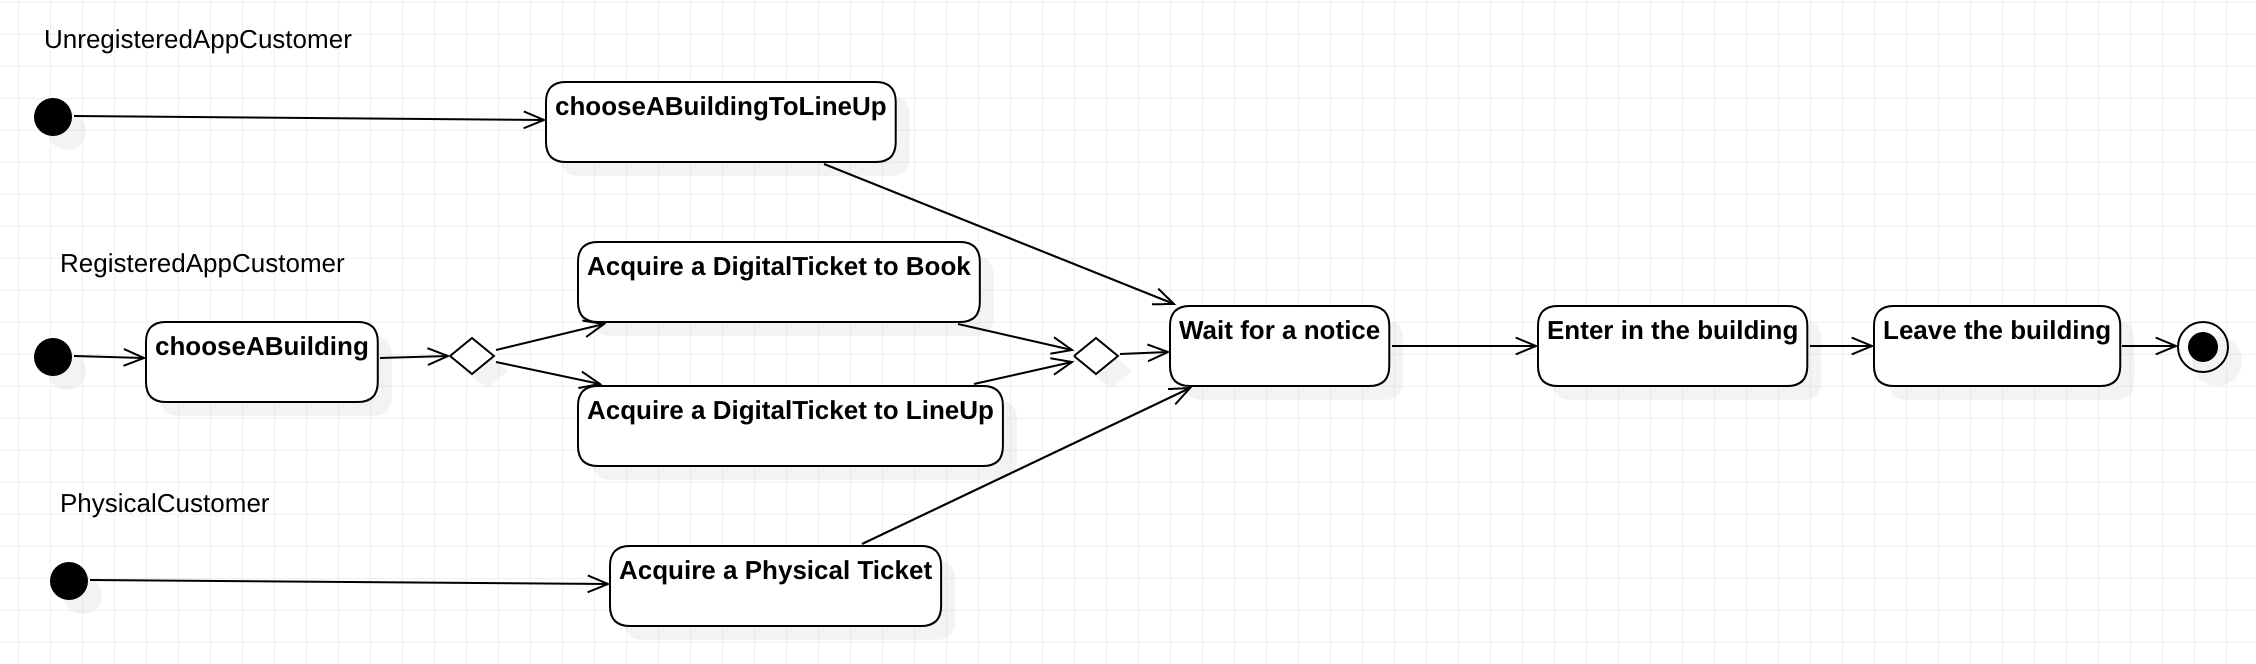
\includegraphics[height=4cm]{ActivityDiagram}\\
	\subsubsection{Use Cases and associated Sequence Diagrams}
	\subsubsection{Mapping table of requirements}
	\subsection{Performance Requirements}
	CLup must guarantee the simultaneous connection of a large number of people, at least x persons, but it can vary according to the performance of the App in the market. Notifications must be sent and delivered in max 10 seconds.
	\subsection{Design Constraints}
	\subsubsection{Standards Compliance}
	No particular standard is required to develop this system.
	\subsubsection{Hardware Limitations}
	Store Manager devices must necessarily have a camera in order to scan Customers’ QR codes. There are no other hardware limitations since the interfaces are quite simple.
	\subsubsection{Any other constraint}
	All the Actors must have a stable internet connection for their mobile device used to access CLup.
	\subsection{Software System Attributes}
         \subsubsection{Reliability}
         The system must be available 24/7, except for any short unexpected interruption, that would not be so serious as long as it lasts for at most a few minutes.
         \subsubsection{Availability}
         The system should be able to respond quickly to faults and to have a fast recovery since building management would be suspended in case of service interruption. Therefore, there must be personnel ready to solve any unexpected issue. All the Actors using the App have to be notified when a system failure occurs.
         \subsubsection{Security}
         The credentials of AppCustomers, Activities and StoreManagers will be stored by CLup, but they must be kept safe, preventing anyone from accessing them. Also any other information, such as AppCustomers position or P.Iva, will be visible only to the system.
         \subsubsection{Maintainability}
         The implementation of the system must guarantee that small adjustments can be made in an easy way. The system has to have a high maintainability especially in order to face possible variations in the number of requests. To do so, the code must be properly commented and organized, avoiding hard-coding.
         \subsubsection{Portability}
         The system will be developed as a mobile App for the main operative systems,  Android and iOS. (?)
	\section{Formal analysis using Alloy}
	<This section should include a brief presentation of the main objectives driving the formal modeling activity, as well as a description of the model itself, what can be proved with it, and why what is proved is important given the problem at hand. To show the soundness and correctness of the model, this section can show some worlds obtained by running it, and/or the results of the checks performed on meaningful assertions.>
	\section{Effort Spent}
	\section{References}
  
\end{document}
